%%%%%%%%%%%%%%%%%%%%%%%%%%%%%%%%%%%%%%%%%%%%%%%%%%%%%%%%%%%%%%%%%%%
%%% Documento LaTeX 																						%%%
%%%%%%%%%%%%%%%%%%%%%%%%%%%%%%%%%%%%%%%%%%%%%%%%%%%%%%%%%%%%%%%%%%%
% Título:		Capítulo 2
% Autor:  	Ignacio Moreno Doblas
% Fecha:  	2014-02-01
% Versión:	0.5.0
%%%%%%%%%%%%%%%%%%%%%%%%%%%%%%%%%%%%%%%%%%%%%%%%%%%%%%%%%%%%%%%%%%%
\chapterbegin{Implementación}
\label{chp:Impl}
%\minitoc

\section{Análisis de requisitos}
\label{sec:Requirements}

Para el desarrollo de este proyecto se han tenido en cuenta una serie de requisitos previos mínimos, necesarios para una correcta implementación del mismo. Los requisitos funcionales de la aplicación fueron acordados en los siguientes:

\begin{itemize}

\item Capacidad de medir la magnitud del ruido ambiente

El usuario debe de ser capaz de realizar mediciones de magnitud del ruido ambiente bajo demanda, así como pararlas a discrección.

\item Capacidad de determinar la posición del dispositivo

La aplicaciónd debe de ser capaz de determinar la posición geográfica del dispositivo con una precisión suficiente para ser utilizada en el posterior procesado de los datos.

\item Capacidad de asociar ambas mediciones

Cada medición de magnitud del ruido ambiente debe de ir acompañada por la posición geográfica en la cual se realizó la misma. 

\item Capacidad de almacenar los datos obtenidos

Los datos recabados en cada sesión de medición deben de ser almacenados de alguna manera para la posterior disponibilidad de estos a discrección del usuario.

\item Capacidad de mostrar los datos obtenidos sobre un mapa

Los datos obtenidos deberán de poder ser representados sobre un mapa geográfico de una manera clara y concisa.

\end{itemize}


Adicionalmente, los siguientes requisitos no funcionales fueron considerados:

\begin{itemize}
\item Extensibilidad futura

La aplicación debe de ser fácilmente extensible en un futuro. Para ello se tendrá en mente la modularidad y el código autoexplicativo durante el desarrollo de la aplicación 

\item Tolerancia a fallos

La aplicación debe de tolerar pequeños fallos sin que estos entorpezcan en medida alguna la posible medición en curso.

\item Rendimiento

La aplicación no debe de ser una carga importante para el rendimiento del sistema, ya que esto podría resultar en mediciones imprecisas o pérdida de muestras por incapacidad del sistema de copar con la carga.

\item Usabilidad

La aplicación está enfocada hacia la accesibilidad de las mediciones de ruido ambiente hacia un público más amplio, por tanto no deberá de ser de dificultoso manejo.

\end{itemize}
\subsection{Diseño de la interfaz gráfica}

Como paso previo a la implementación en código, se han diseñado unos borradores de las distintas pantallas de las que constará la aplicación. La aplicación se ha dividido en cuatro pantallas básicas: mapa, grabar, sesiones y opciones, las cuales se pueden observar en la figura \ref{fig:mockup}.

\begin{description}
\item[Mapa] es la pantalla inicial, que muestra un mapa geográfico y nos permite superponer los datos previamente recabados
\item[Grabar] es la pantalla que interactúa con los sensores del dispositivo y comanda las acciones de grabación y guardado de archivos.
\item[Sesiones] presenta todos los datos recabados en pasadas grabaciones.
\item[Opciones] permite ajustar los parámetros que en la aplicación hayan sido decididos como configurables.
\end{description} 

\begin{figure}[h] \centering
    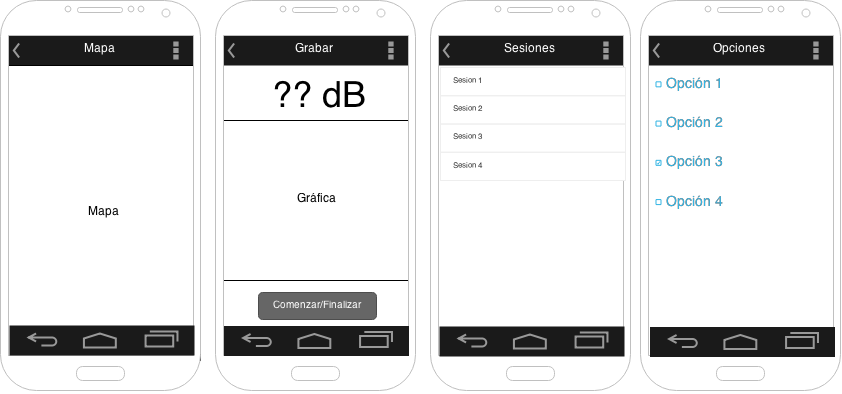
\includegraphics[width=15cm]{graphs/mockup.png} \caption{Primer borrador sobre el aspecto de las distintas pantallas de la aplicación}\label{fig:mockup}
\end{figure}
\subsection{Dispositivo Android}

El desarrollo de este proyecto ha sido realizado y testeado en dos dispositivos. El primero, modelo HTC Desire HD poseedor de la versión 4.2.2 de Android y el segundo Google Nexus 5, bajo la versión Android 5.0, lo cual garantiza que la aplicación conserva toda su funcionalidad en los modelos más modernos, tanto en software como en hardware. 

No obstante, también se ha comprobado su funcionalidad en una rango de dispositivos más amplio, tales como Samsung Galaxy S3, Samsung Galaxy Nexus, Sony Xperia P, no mostrando pérdida alguna de funcionalidad.

La versión mínima de Android requerida para el correcto funcionamiento de esta aplicación, es el nivel de \ac{API} 15, correspondiente a Android 4.0.3. Es posible hacerla funcionar en niveles más bajos (antiguos), pero requiere esfuerzo adicional, tal y como se esboza en el apartado de Conclusiones y Trabajo Futuro.

\subsection{Micrófono externo}

Los micrófonos empotrados en los teléfonos móviles tienen un objetivo muy claro y marcado, que es la transmisión de voz vía redes celulares, y muestran cierto sesgo en diseño cuando se les intenta usar para otro propósito.

Un perfecto ejemplo de ello es el \ac{CAG}. El \ac{CAG} es de verdadera utilidad para mejorar los niveles sonoros realizando una llamada, pero entra en conflicto con el propósito de este proyecto, ya que necesita de una señal sin pre-procesamiento alguno. El efecto de compresión que realiza el \ac{CAG}, proporciona unas medidas sin sentido alguno.

Adicionalmente, el tamaño y posición empotrada del mismo, los hace muy sensibles a interferencias indeseadas tales como la vibración del propio teléfono.

Uno de los modelos utilizados en el desarrollo, el Google Nexus 5, permite la desactivación del \ac{CAG}, por tanto se obtienen medidas aceptables. No obstante, para mejores resultados, se debe de usar un micrófono externo sin \ac{CAG}.

\subsection{Calibración}
La aplicación debe de ser capaz de adaptarse a distintos dispositivos, y no sólo trabajar correctamente con el dispositivo en el que fue desarrollada. Para ello, se habilita en las opciones de la aplicación un apartado en el que se pueda introducir un valor de compensación en la medida. Esto ayuda a subsanar previsibles diferencias entre los sistemas de captación sonora de distintos dispositivos móviles.

\section{Aplicación Android}

\subsection{Herramientas de desarrollo}


\subsection{Estructura del código}

La estructura de la aplicación sigue la estructura estándar de proyecto Android que se sigue en el entorno de desarrollo Android Studio. Se distinguen cuatro grupos principales:
\begin{description}
\item[Manifiestos] son archivos que presentan la aplicación al sistema operativo y proveen información básica sobre la misma, tal como el paquete Java de la aplicación, los componentes de la misma (actividades, servicios, eventos de emisión, proveedores de contenido...), los permisos requeridos por la aplicación, el nivel mínimo de \ac{API} Android requerido y los permisos proporcionados por la aplicación.
\item[Código fuente] escrito en el lenguaje de programación Java, el cual será compilado posteriormente y convertido a código intermedio. Toda la lógica de la aplicación está implementada de esta manera. El código fuente a su vez se organiza dentro de paquetes, que son agrupaciones lógicas y funcionales de distintos archivos de código fuente.
\item[Recursos] que incluyen todo elemento gráfico, diseño de interfaces gráficas de usuario o componentes de las mismas, composición de menús contextuales, y valores de variables. Es posible proveer distintas versiones de cada uno de los recursos enfocadas a características en concreto de los dispositivos. Por ejemplo, es posible especificar un recurso para un idioma del télefono, tamaño de pantalla, ratio, orientación del dispositivo, versión de la API Android e incluso si el dispositivo se encuentra en modo nocturno o no.
\item[Instrucciones de compilación] escritos en el \ac{DSL} de Gradle. Esto es una herramienta de automatización de proyectos que permite manejar de manera cómoda y eficiente tareas como gestión de dependencias, compilación, empaquetado y publicado de artefactos.
\end{description}
 
 A su vez, el código fuente está dividido en subpaquetes. Se ha creado un paquete para las actividades, otro paquete para los fragmentos, otro paquete para los servicios y un último paquete para las clases de utilidad y misceláneas. Dicha estructura puede observarse en la figura \ref{fig:srctree}.
 
 \begin{figure}[h] \centering
    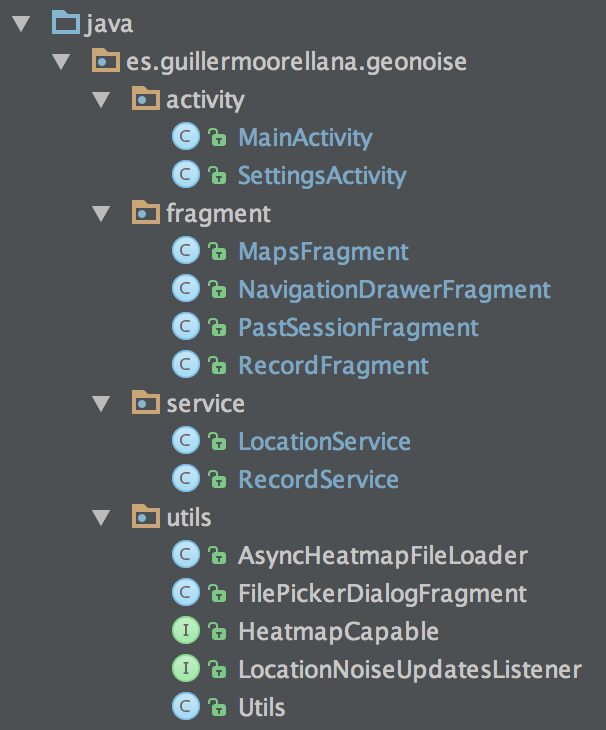
\includegraphics[height=10cm]{graphs/srctree.png} \caption{Organización del código fuente.}\label{fig:srctree}
\end{figure}
 
\subsection{Interfaz gráfica}

La interfaz gráfica de esta aplicación se ha desarrollado siguiendo las guías de diseño vigentes para la versión del sistema KitKat. Estas no son las más modernas, ya que recientemente han sido actualizadas a Lollipop, y las guías de diseño cambiadas hacia el llamado “Material Design” (diseño material), pero se ha desestimado seguirlas dadas su novedad, que implica una nueva curva de aprendizaje y posible escasez de recursos de apoyo.

No obstante, la interfaz es sencilla e intuitiva, y resulta familiar para todo usuario del sistema operativo Android. Además se han incluido explicaciones y guías de usuario dentro de la aplicación, para mejorar su usabilidad y asegurar el correcto uso de la misma por parte del usuario.

En Android hay dos maneras de definir una interfaz gráfica: programáticamente o por archivos de recurso XML. Se ha optado por la segunda opción, la cual disminuye el acoplamiento en el código, aumenta la reusabilidad y la claridad del mismo, y por otra parte el entorno de desarrollo permite previsualizar el resultado de dichos archivos XML con bastante fidelidad.

 \begin{figure}[hb] \centering
    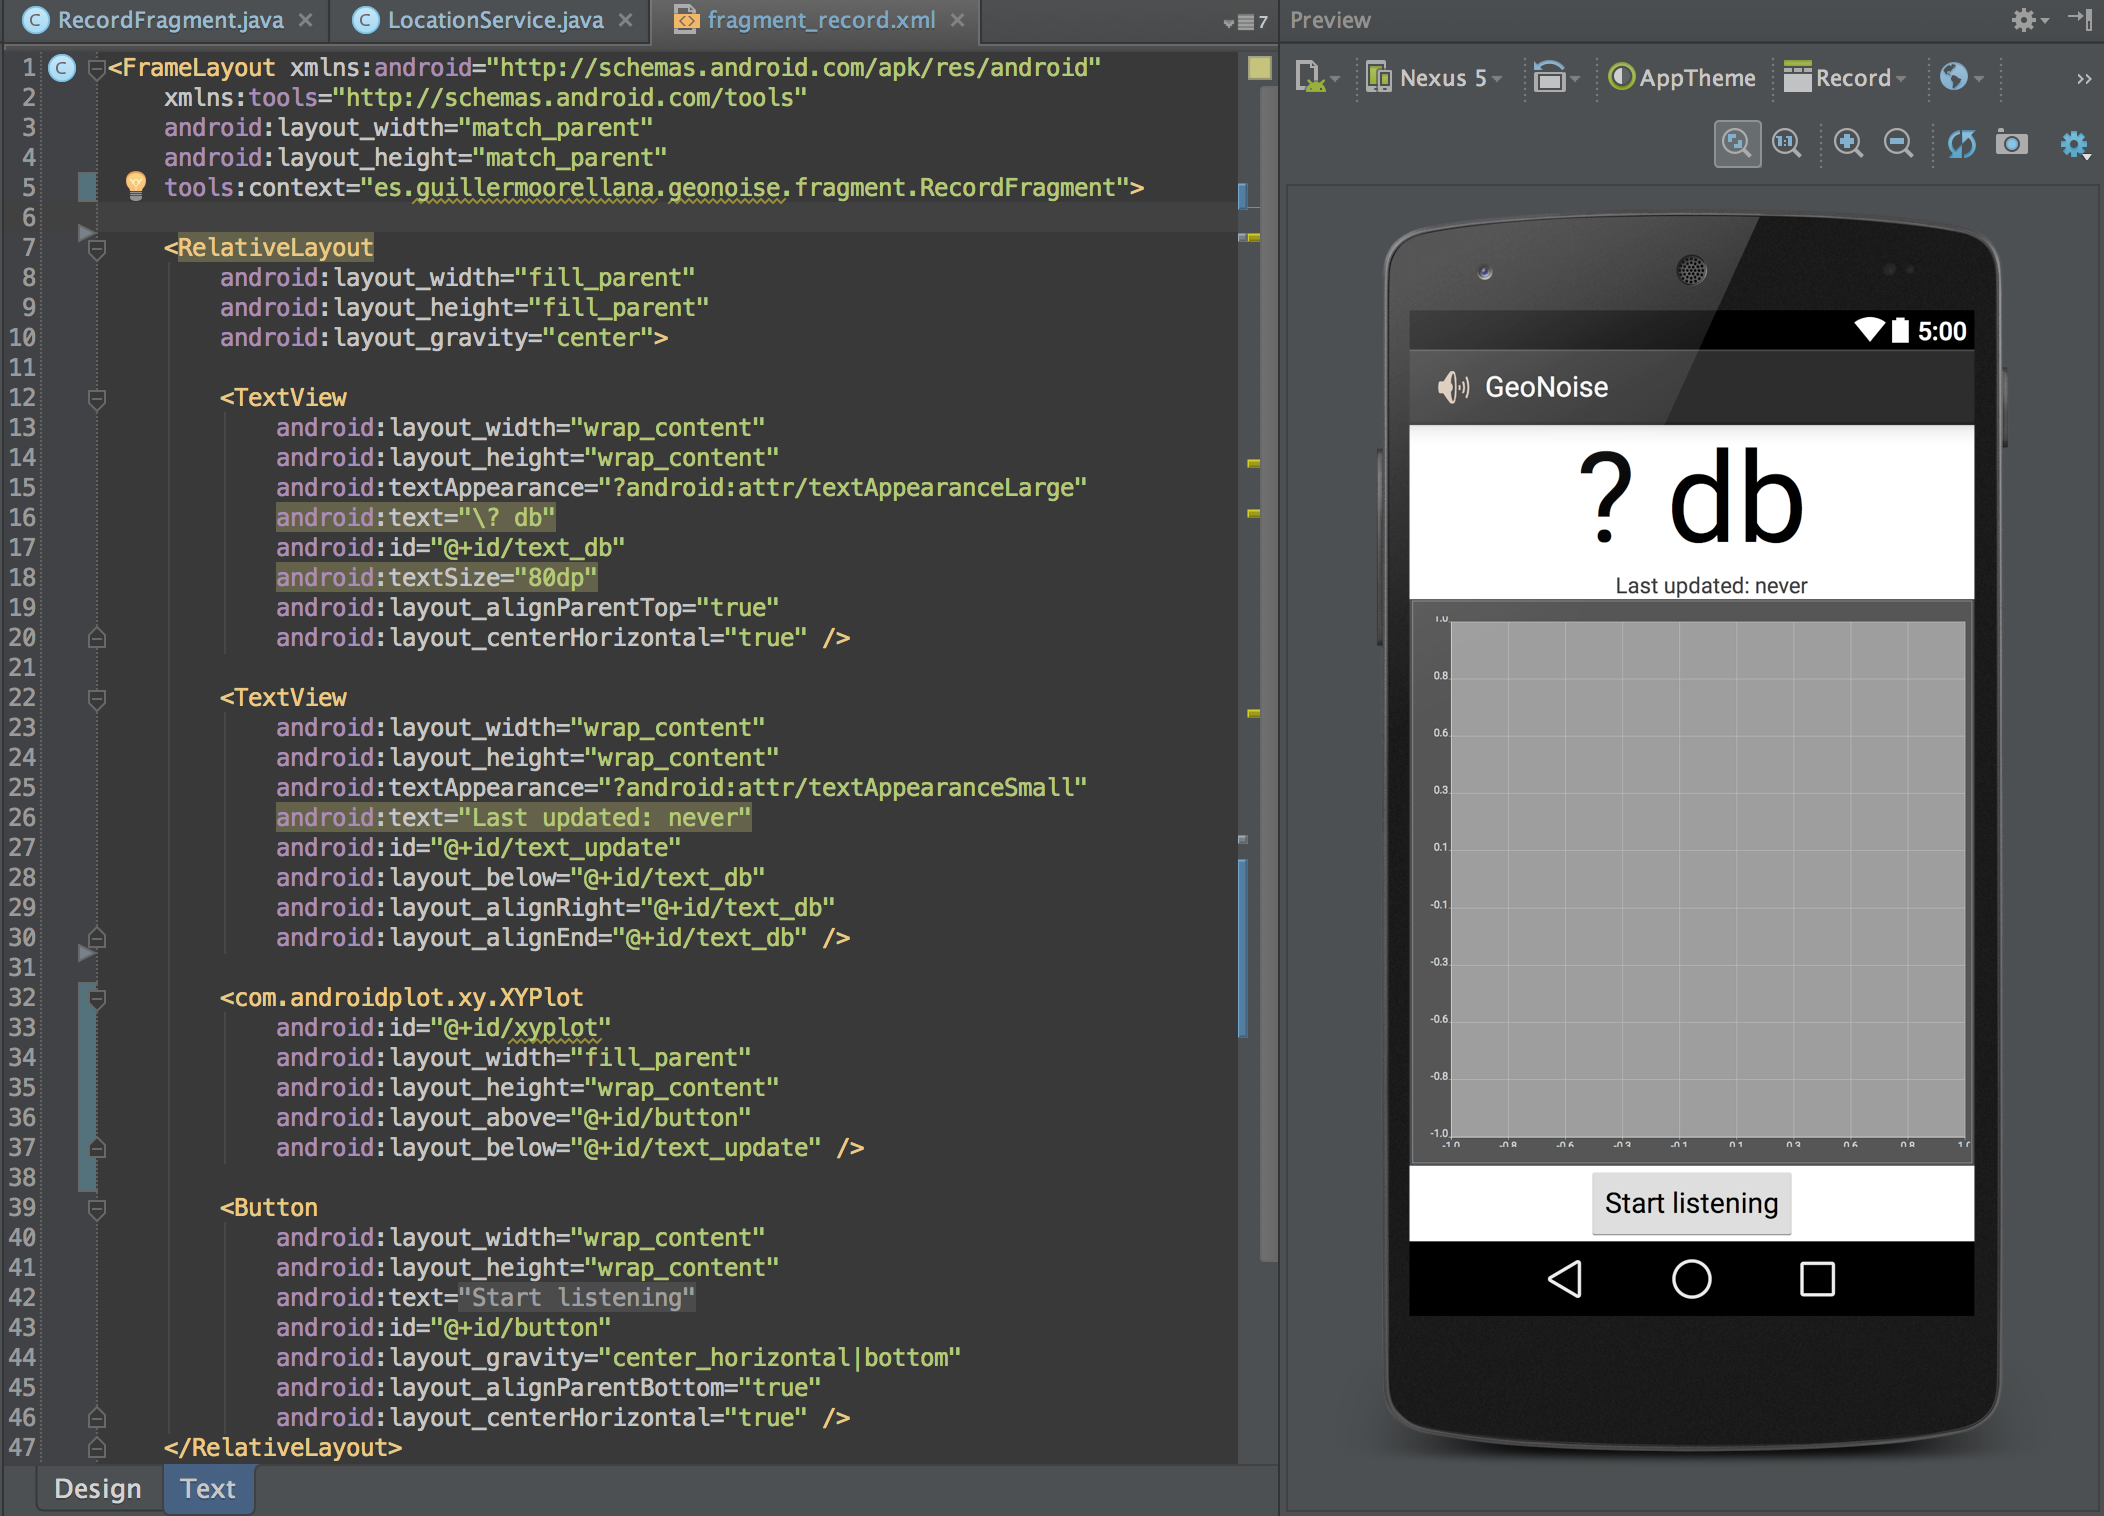
\includegraphics[height=10cm]{graphs/layoutedit.png} \caption{Editor de archivos de recurso XML con vista previa.}\label{fig:layoutedit}
\end{figure}

Además, en consonancia con las últimas recomendaciones de diseño de aplicaciones de Google, se han utilizado fragmentos cuando ha sido conveniente, incrementando la modularidad de los componentes de la interfaz gráfica y su potencial reusabilidad.

Para el diseño de los archivos XML se ha hecho uso de la herramienta incorporada para tal propósito en el entorno de desarrollo Android Studio, la cual nos brinda la posibilidad de tener una vista previa del resultado de la descripción en XML que estamos realizando dela interfaz gráfica de usuario. Como ejemplo, en la figura \ref{fig:layoutedit} se puede observar la edición de la interfaz gráfica de usuario de la actividad engargada de grabar los sonidos.

Si así se deseara, también cambe la posibilidad de diseñar las interfaces gráficas de usuario de la aplicación mediante la misma herramienta, pero de una manera completamente visual, tal y como se observa en la figura \ref{fig:layoutvisual}. De esta manera, se sacrifica precisión y control por comodidad y claridad.

 \begin{figure}[H] \centering
    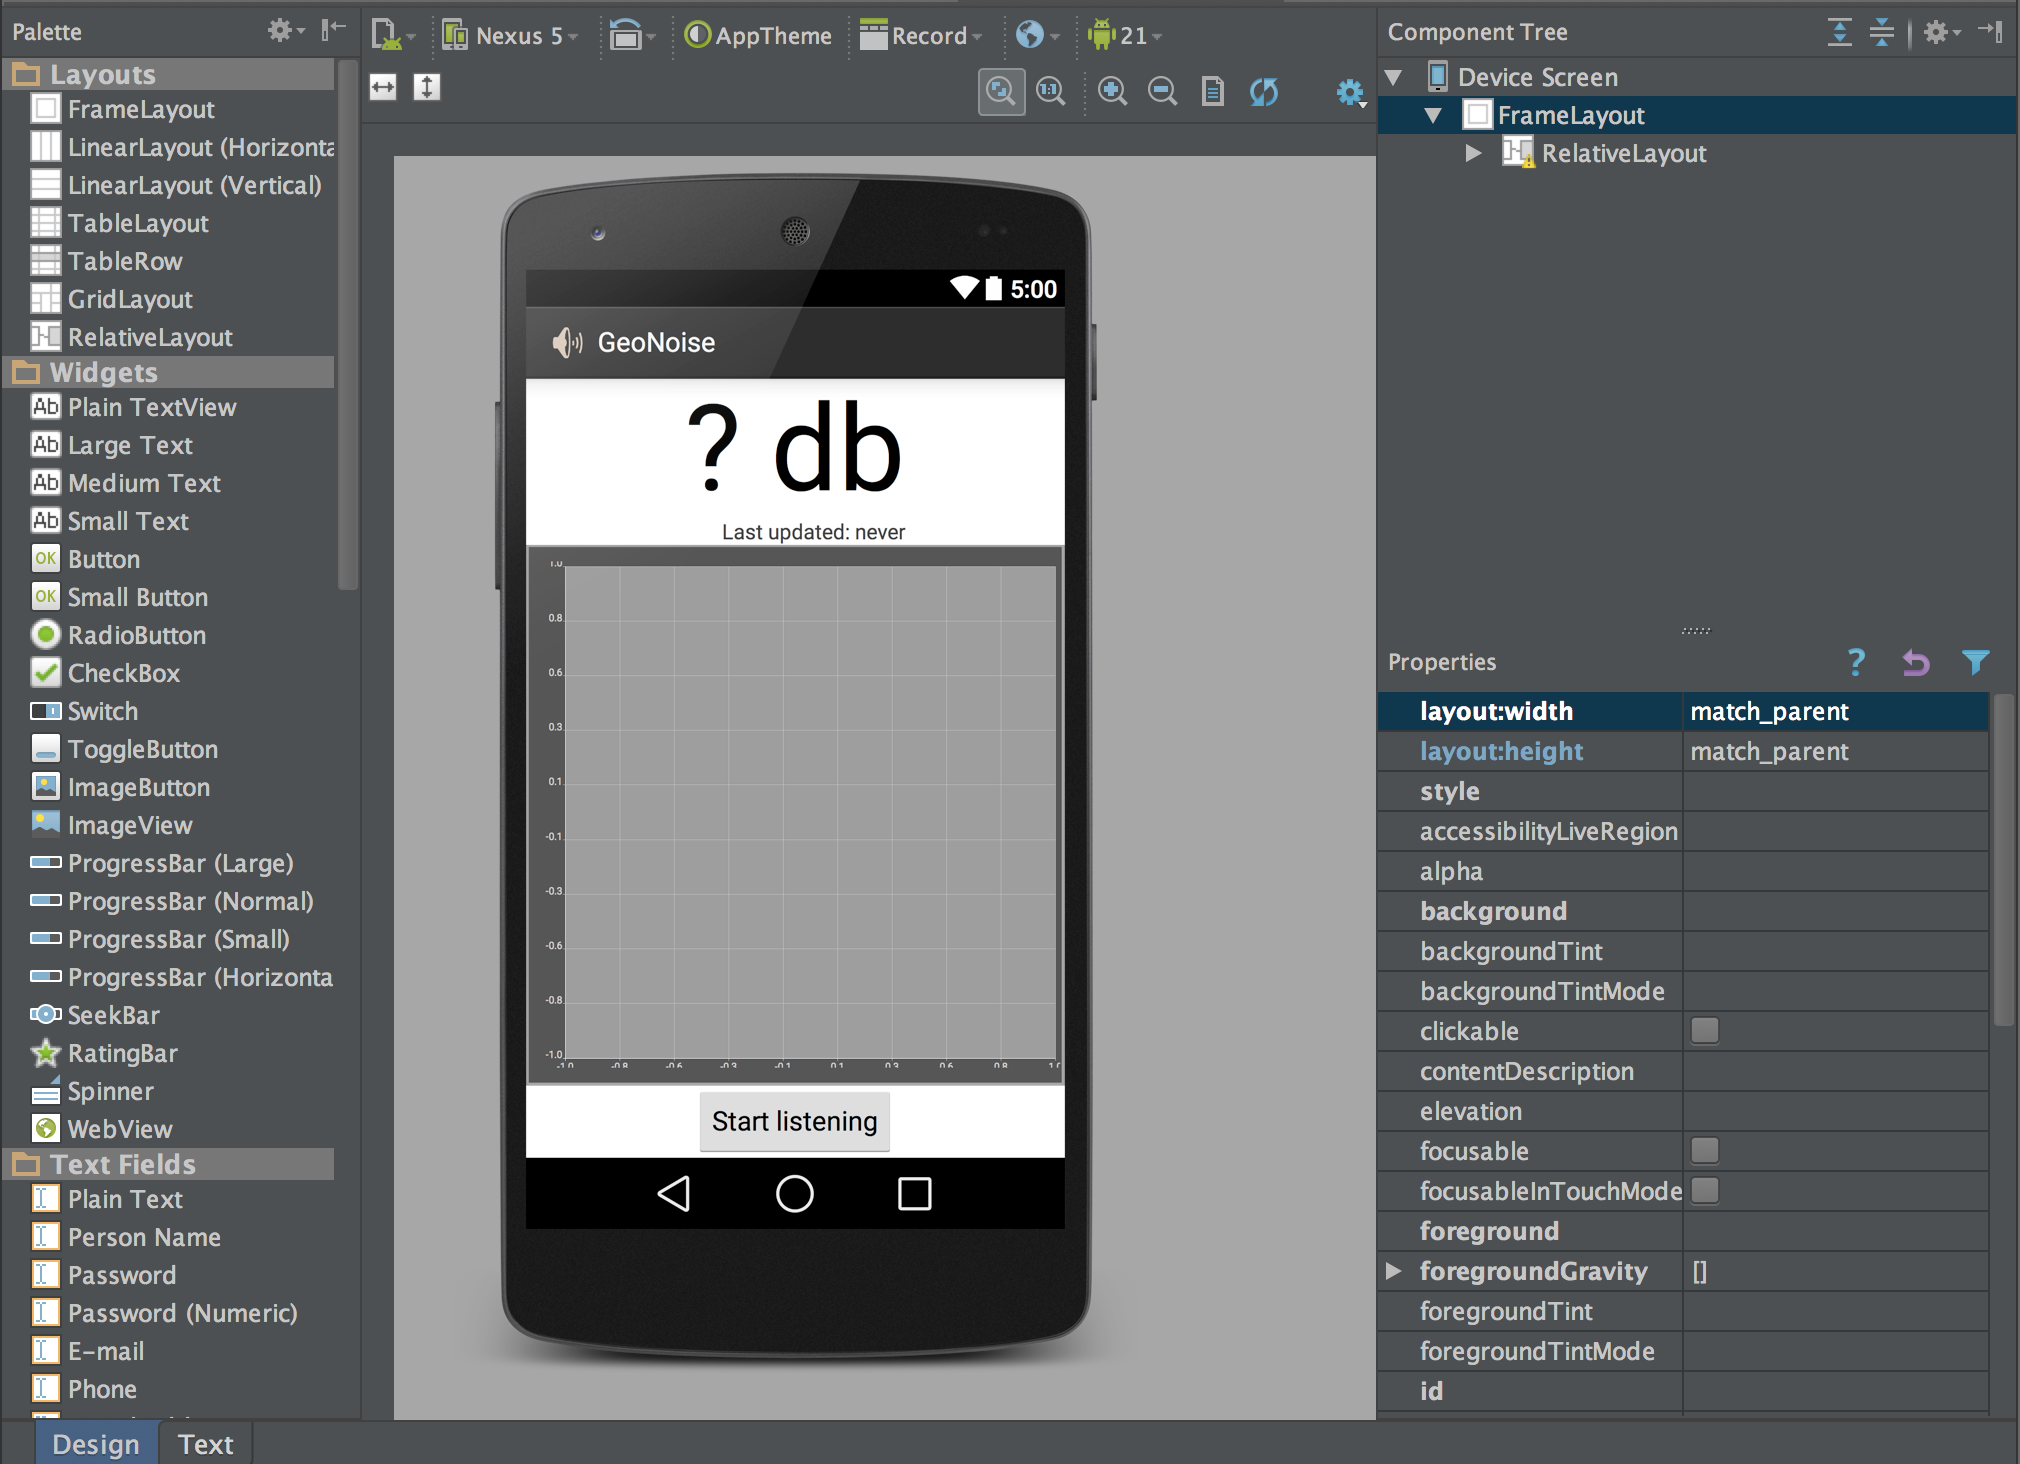
\includegraphics[height=10cm]{graphs/layoutvisual.png} \caption{Edición completamente visual de la interfaz gráfica de usuario de la aplicación.}\label{fig:layoutvisual}
\end{figure}

Dentro de cada pantalla, la estructuración de los elementos que se observan se realiza a través de layouts. Los layouts pueden definirse como contenedores de una o más vistas, que ayudan al posicionamiento de cada una de ellas dentro de la aplicación así como a controlar el comportamiento de las mismas. Este concepto encaja a la perfección con el anidado de etiquetas de XML. En el ejemplo de la figura \ref{fig:layoutedit}, el código XML es el presente en el extracto \ref{code:layout}. En dicho extracto se puede observar cómo el elemento \ttw{RelativeLayout} contiene a varios elementos a su vez, entre otros \ttw{TextView} y \ttw{Button}, y cómo estos elementos interiores definen su posición y tamaño en relación al resto de elementos. 

\begin{figure}[H] 
%\RecustomVerbatimEnvironment{Verbatim}{BVerbatim}{}
\begin{minted}[linenos,numberblanklines,breaklines,frame=lines]{xml}
<RelativeLayout
    android:layout_width="fill_parent"
    android:layout_height="fill_parent"
    android:layout_gravity="center">
    <TextView
        android:layout_width="wrap_content"
        android:layout_height="wrap_content"
        android:text="\? db"
        android:id="@+id/text_db"
        android:textSize="80dp"
        android:layout_alignParentTop="true"
        android:layout_centerHorizontal="true" />
    <TextView
        android:layout_width="wrap_content"
        android:layout_height="wrap_content"
        android:text="Last updated: never"
        android:id="@+id/text_update"
        android:layout_below="@+id/text_db"
        android:layout_alignRight="@+id/text_db"
        android:layout_alignEnd="@+id/text_db" />
        [...]
</RelativeLayout>
\end{minted}
\caption{Preparación de AudioRecord}
\label{code:layout}
\end{figure}

\subsubsection{Cajón de Navegación}
El cajón de navegación, más conocido por su denominación inglesa Navigation Drawer, es un patrón de interfaz de usuario muy utilizado en Android. Consiste en un panel que transiciona desde el borde izquierdo de la pantalla y muestra las opciones principales de navegación de la aplicación. Se ha decidido incluir dicho patrón de diseño en la aplicación dado que permite una mejor utilización del espacio, al no bloquear región alguna de la pantalla mientras se encuentra sin desplegar.

 \begin{figure}[H] \centering
    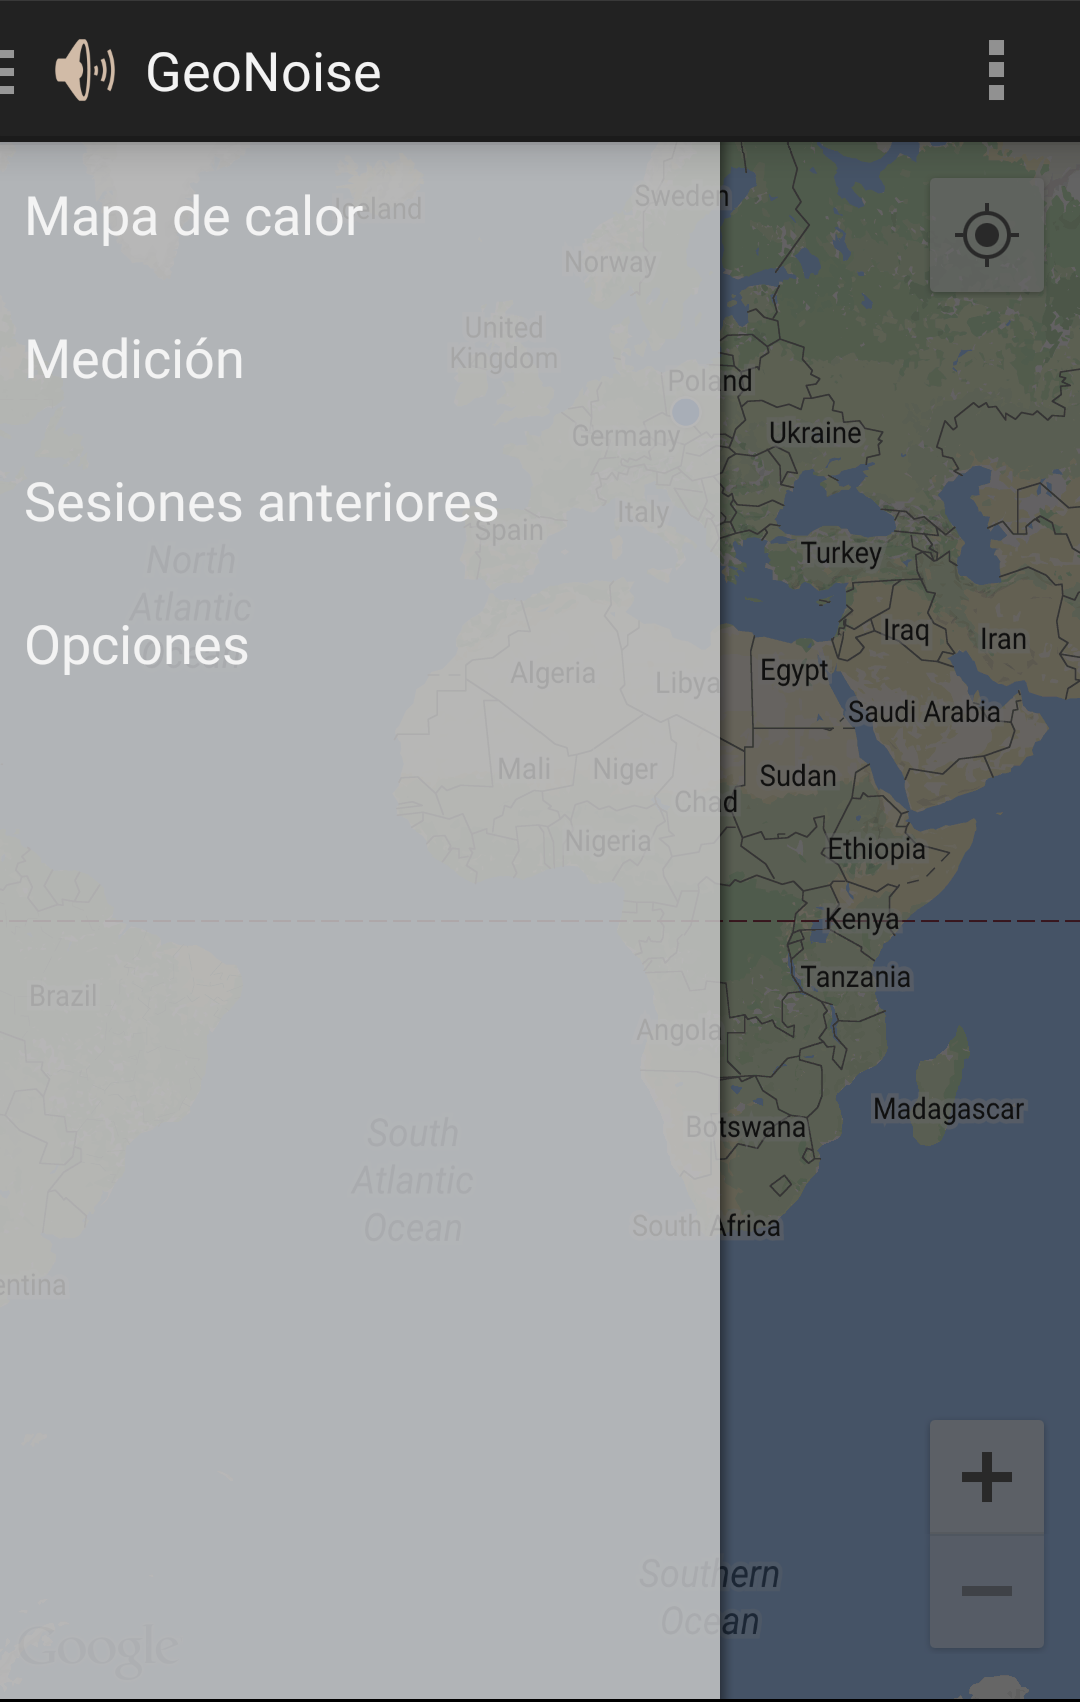
\includegraphics[height=10cm]{graphs/navdrawer.png} \caption{Patrón de cajón de navegación implementado en la aplicación.}\label{fig:navdrawer}
\end{figure}

\subsection{Captura de audio}

El sistema operativo Android provee una \ac{HAL} que conecta todas las \ac{API} de alto nivel con los controladores y hardware subyacentes en cada dispositivo. La figura \ref{fig:diagrama:audiohal} muestra los distintos niveles de la arquitectura del audio en el sistema operativo Android y su interconexión.
\begin{figure}[h] \centering
    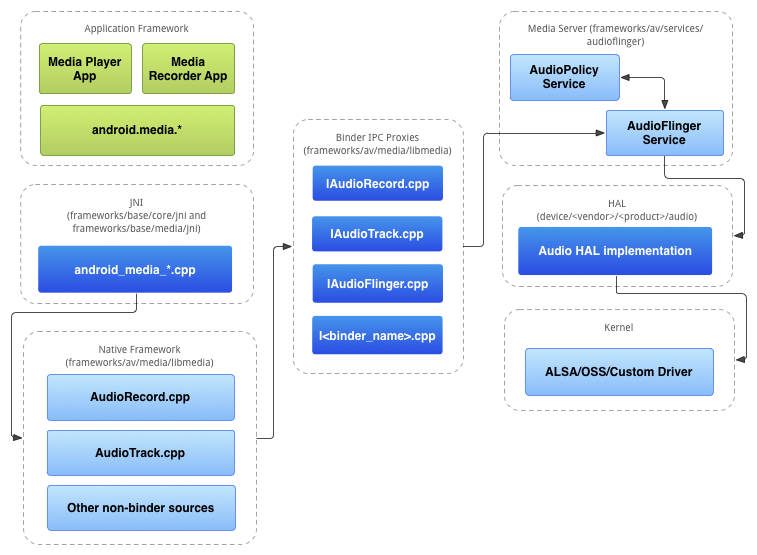
\includegraphics[height=10cm]{graphs/audio_hal.png} \caption{Arquitectura del audio en Android. Tomado de \cite{audiohal}}\label{fig:diagrama:audiohal}
\end{figure}

En la aplicación se ha optado por la simplicidad, y utilizado las clases del paquete \ttw{android.media.*} que provee el framework, y que brindan un nivel de abstracción bastante cómodo.

Para garantizar que la operación de captura de audio no se ve interferida por otras funciones de la aplicación, se ha optado por crear un servicio que corra en segundo plano y responda a los comandos de la aplicación en primer plano, tal y como se explicó en el apartado \ref{ssec:teo:svc}.

El servicio hace uso de la clase \ttw{AudioRecord}, la cual requiere una preparación previa a la grabación, tal y como se muestra en el extracto \ref{code:audioprep}.

\begin{figure}[h] 
%\RecustomVerbatimEnvironment{Verbatim}{BVerbatim}{}
\begin{minted}[linenos,numberblanklines,breaklines,frame=lines]{java}
private void prepareAudio() {
    try {
        bufferSize = 10 * AudioRecord.getMinBufferSize(sampleRate, AudioFormat.CHANNEL_IN_MONO, AudioFormat.ENCODING_PCM_16BIT);
        samplePeriod = 1.0f / ((float) sampleRate / (float) bufferSize);
        audio = new AudioRecord(MediaRecorder.AudioSource.VOICE_RECOGNITION, sampleRate, AudioFormat.CHANNEL_IN_MONO, AudioFormat.ENCODING_PCM_16BIT, bufferSize);
    } catch (Exception e) {
        Log.d(TAG, "Error creating audioRecorder");
    }
}
\end{minted}
\caption{Preparación de AudioRecord}
\label{code:audioprep}
\end{figure}

Una vez la instancia de AudioRecord ha sido configurada, es posible comenzar la misma llamando al método \ttw{startRecording()}. De esta manera, el sistema operativo empezará a rellenar el búfer interno de la instancia de AudioRecord según los parámetros que han sido indicados. Los datos del búfer son obtenidos bajo demanda, llamando al método \ttw{read(short[] audioData, int offsetInShorts, int sizeInShorts)} que introducirá en el búfer referenciado las muestras obtenidas hasta el momento. Una muestra de cómo es realizado en la aplicación está presente en la figura \ref{code:audiocapture}. 

Las muestras están codificadas en formato \ac{PCM} de 16 bits con signo. Por tanto, el límite superior del valor de las muestras es $2^15-1=32767$. Los teléfonos móviles inteligentes suelen incorporar micrófonos de tecnología \ac{MEMS}. El valor típico de saturación de estos micrófonos es de 90dB SPL. Asumiremos pues, que el valor máximo \ttw{32767} corresponde a 90dB SPL, que corresponden con $0.6325 Pa$ en el micrófono. Asumiremos también que para el valor $P_0=0.00002 Pa$ se obtiene una muestra PCM con valor 1.
En consecuencia, a las muestras obtenidas les es aplicado un factor $\frac{32767}{0.6325 Pa} =  51805.5336 Pa^{-1}$.

\begin{figure}[h] 
%\RecustomVerbatimEnvironment{Verbatim}{BVerbatim}{}
\begin{minted}[mathescape,linenos,numberblanklines,breaklines,frame=lines]{java}
short[] buffer = new short[bufferSize];
int resultSize = -1;
resultSize = audio.read(buffer, 0, bufferSize);
double sum = 0;
// $ p_\mathrm{rms} = \left[ \frac{1}{T} \int_0^T p^2(t)dt \right]^\frac{1}{2} = \left( \frac{1}{T} \sum\limits_0^T p^2[n] \right)^\frac{1}{2} $
for (int i = 0; i < resultSize; i++) {
    sum += buffer[i] / 51805.5336 * buffer[i] / 51805.5336;
}
double p_rms = Math.sqrt(sum / resultSize);
\end{minted}
\caption{Captura de muestras con AudioRecord y cálculo de la $p_{rms}$}
\label{code:audiocapture}
\end{figure}

Al mismo tiempo que se realiza la captura de sonido, se solicita al servicio de geolocalización la posición actual, para poder relacionar ambas medidas. Dicho servicio de geolocalización se trata en detalle en la sección \ref{sec:impl:geo}.

Una vez obtenido el contenido del búfer de muestras, realizamos el procesado de las mismas. Según la definición de $p_{rms}$ vista en la ecuación \ref{eq:prms}, y teniendo en cuenta que para muestras discretas la integral pasa a ser un sumatorio, se implementa el cálculo de $p_{rms}$ tal y como en \ref{code:audiocapture}.

El siguiente paso es obtener el \ac{SPL} correspondiente a la $p_{rms}$ calculada, implementado en ka figura \ref{code:spl} según la ecuación \ref{eq:spl}. Se ha añadido una constante \ttw{splAdjustment}, la cual se utiliza para calibrar previsibles diferencias en el sistema captador de audio de distintos teléfonos.

\begin{figure}[h] 
%\RecustomVerbatimEnvironment{Verbatim}{BVerbatim}{}
\begin{minted}[mathescape,linenos,numberblanklines,breaklines,frame=lines]{java}
public double getDecibels(double level) {
    return Math.abs(20.0 * Math.log10(level /  0.00002)) + splAdjustment;
}
\end{minted}
\caption{Cálculo del SPL.}
\label{code:spl}
\end{figure}

\subsection{Geolocalización}
\label{sec:impl:geo}
Para obtener la posición absoluta del dispositivo móvil, la aplicación se comunica con los \ac{GMS}, que no sólo actúan como una capa de abstracción del hardware GPS del dispositivo, sino que además proveen servicios de valor añadido, tales como un menor tiempo de precalentamiento, localización por redes WiFi u optimización del consumo energético.

Se utiliza un servicio en segundo plano por los mismos motivos que en el apartado de Captura de Audio. De hecho, es un servicio intermedio, ya que la obtención en sí de la posición la hace el servicio \ac{GMS}. La interacción de la aplicación con los distintos servicios se puede observar en el diagrama \ref{fig:diagrama:servicios}.

El servicio creado en la aplicación se conecta a los \ac{GMS}, solicita actualizaciones y las pone a disponibilidad del resto de la aplicación de la manera mostrada en \ref{code:location}.

\begin{figure}[h] \centering
\begin{tikzpicture}[node distance = 4cm, auto]
    % Place nodes
    \node [block] (app) {Aplicación};
    \node [block, right of=app] (audio) {Servicio de captura de audio};
    \node [block, right of=audio] (loc) {Servicio de localización};
    \node [block, right of=loc] (gms) {GMS};
    % Draw edges
    \path [line] (app) -- (audio);
    \path [line] (audio) -- (loc);
    \path [line] (loc) -- (gms);
\end{tikzpicture}
\caption{Diagrama de interacción de la aplicación y los servicios.}\label{fig:diagrama:servicios}
\end{figure}

\begin{figure}[h] 
%\RecustomVerbatimEnvironment{Verbatim}{BVerbatim}{}
\begin{minted}[mathescape,linenos,numberblanklines,breaklines,frame=lines]{java}
private GoogleApiClient locationClient;
locationClient = new GoogleApiClient.Builder(this)
        .addApi(LocationServices.API)
        .addConnectionCallbacks(this)
        .addOnConnectionFailedListener(this)
        .build();
locationClient.connect();
\end{minted}
\caption{Solicitud de conexión a los GMS.}
\label{code:location}
\end{figure}

\chapterend{}